\documentclass[aspectratio=169]{beamer}
\usepackage{colortbl}
\usepackage{amsmath}
\usepackage{tikz}

\usepackage[ruled]{algorithm2e}

\usepackage[]{natbib}
\bibliographystyle{abbrvnat}

\makeatletter
\@newctr{footnote}[page]
\makeatother

\usepackage{adjustbox}
\usepackage[utf8x]{inputenc}
\usepackage{graphicx}
\usepackage{subfig}

\usepackage[tikz]{mdframed}
\usepackage{calc}
\usepackage{appendixnumberbeamer}

% \usepackage[perpage]{footmisc}
\renewcommand\thempfootnote{\arabic{mpfootnote}}

\pdfpageattr{/Group <</S /Transparency /I true /CS /DeviceRGB>>}

\usepackage{xcolor}

% MATLAB colors
\definecolor{matlab-blue}{rgb}{0.0000, 0.4470, 0.7410}
\definecolor{matlab-red}{rgb}{0.8500, 0.3250, 0.0980}
\definecolor{matlab-yellow}{rgb}{0.9290, 0.6940, 0.1250}
\definecolor{matlab-purple}{rgb}{0.4940, 0.1840, 0.5560}

% NTNU colors
\definecolor{ntnu-blue}{RGB}{0, 80, 158}

% SINTEF colors
% \definecolor{sintef-green}{RGB}{0,172,160}
\definecolor{sintef-gray}{RGB}{51,51,51}
\definecolor{sintef-blue}{RGB}{0,61,101}

% Phase colors
\definecolor{aqu}{RGB}{95 ,  95, 211}
\definecolor{liq}{RGB}{145, 124, 111}
\definecolor{rock}{RGB}{179, 179, 179}

% Code
\colorlet{codecolor}{matlab-yellow!6}

\mdfsetup{
  tikzsetting = {fill = ye!10},
  linecolor = black,
  roundcorner=4pt,
  linewidth=1.5pt,
  userdefinedwidth=0.5\linewidth,
}

\newlength{\frameheight}
\setlength{\frameheight}{0.9\textheight}

\mode<presentation>
{

\setbeamercolor{section in toc}{fg=black,bg=white}
\setbeamercolor{alerted text}{fg=black!80!gray}
\setbeamercolor*{palette primary}{fg=white,bg=sintef-blue}

\setbeamercolor{titlelike}{parent=palette primary,fg=white}
\setbeamercolor{frametitle}{bg=sintef-blue}
\setbeamercolor{frametitle right}{bg=gray!60!white}

\setbeamercolor*{separation line}{}
\setbeamercolor*{fine separation line}{}

\useinnertheme[shadow=false]{rounded}

\setbeamercolor*{block title}{bg = sintef-blue, fg = white}
\setbeamercolor*{block body}{bg = sintef-blue!20, fg = black}

}

\setbeamertemplate{navigation symbols}{}
\setbeamertemplate{footline}[frame number]
\setbeamerfont{block title}{size={},series=\bfseries}
\def\Tiny{\fontsize{5pt}{5pt}\selectfont}
\setbeamertemplate{enumerate items}[default]

\usetikzlibrary{arrows,shapes,positioning,shadows,calc,tikzmark,arrows,decorations.pathreplacing}
% \captionsetup[subfigure]{labelformat=empty}
\captionsetup[figure]{labelformat=empty}

\usepackage[absolute,overlay]{textpos}

\definecolor{bl}{rgb}{0     , 0.4470, 0.7410}
\definecolor{re}{rgb}{0.8500, 0.3250, 0.0980}
\definecolor{ye}{rgb}{0.9290, 0.6940, 0.1250}
\definecolor{alertclr}{rgb}{0.8500, 0.3250, 0.0980}

\newcommand{\redtext}[1]{\textcolor{matlab-red}{#1}}
\newcommand{\graytext}[1]{\textcolor{black!20}{#1}}
\newcommand{\bluetext}[1]{\textcolor{matlab-blue}{#1}}

\tikzstyle{explain} = [rectangle, draw = black, fill=ye!10, rounded corners, font = \small, thick, text centered, minimum height = 1.7em, align = left]
\tikzstyle{pointer} = [<-, line width = 1pt]

\usepackage{enumitem}
\newenvironment{squarelist}
{
    \begin{enumerate}
    [
    label={\raisebox{.15ex}{\protect\textcolor{sintef-blue}{\tiny$\blacksquare$}{\protect}}},
    labelindent = 0.3em,
    leftmargin = *,
    align = left
    ] 
}
{
  \end{enumerate}
}

\newenvironment{circlelist}
{
    \begin{enumerate}
    [
    label={\raisebox{.15ex}{\protect\textcolor{sintef-gray}{$\bullet$}{\protect}}},
    labelindent = 0.3em,
    leftmargin = *,
    align = left
    ] 
}
{
  \end{enumerate}
}

\newenvironment{numlist}
{
  \begin{enumerate}
    [
    label=\protect\textcolor{sintef-gray}{\arabic*.},
    labelindent = 0.3em,
    leftmargin = *,
    align = left
    ] 
}
{
  \end{enumerate}
}

\newenvironment{vertlist}
{
  \begin{enumerate}
    [
    label=\protect\textcolor{sintef-gray}{$\lvert$},
    labelindent = 0.3em,
    leftmargin = *,
    align = left
    ] 
}
{
  \end{enumerate}
}

\newcommand{\mycite}[1]{\footnote{#1}}

\usepackage{listofitems}
\newcommand{\myfootcite}[1]{%
    \footnote{%
        \foreach \k in {#1}{
            \citeauthor{\k}, \citeyear{\k}.
        }
    }%
}

\newcommand{\un}{u}
\newcommand{\expect}{\mathbb{E}}
\newcommand{\expecta}{E}
\newcommand{\var}{\mathbb{V}}
\newcommand{\vara}{V}
\newcommand{\nsamp}{N}
\newcommand{\nlev}{L}
\newcommand{\cost}{C}

\newcommand{\Oh}{\mathcal{O}}
\newcommand{\err}{\mathcal{E}}
\newcommand{\tol}{\varepsilon}

\newcommand{\mc}{{\mathsf{MC}}}
\newcommand{\ml}{{\mathsf{ML}}}

\usepackage{bm}
\newcommand{\vect}[1]{\bm{#1}}
\newcommand{\vel}{\vec v}
\newcommand{\perm}{K}
\newcommand{\vx}{\vect x}
\newcommand{\spa}{D}
\newcommand{\bhp}{p_{\mathsf{bh}}}
\newcommand{\dd}{\mathsf{d}}

\newlength{\cw}
\setlength{\cw}{0.5\textwidth}


\title{Multilevel Monte Carlo Methods for Uncertainty Quantification in Reservoir Simulation}

\author[Ø.S. Klemetsdal]{Øystein S. Klemetsdal}%
% \institute[SINTEF]{Department of Mathematics and Cybernetics, SINTEF Digital, Norway}%
\date[27/11/19]{PhD Trial Lecture\\November 27, 2019, NTNU, Trondheim, Norway}%

\begin{document}

\maketitle

\nocite{*}

\section{Introduction}
\def\name{Introdution}
\begin{frame}{\name{}}
    \begin{squarelist}
        \item<1-> Many problems are in principle deterministic, but we don't know the parameters
        \begin{circlelist}
            \item From computational finance to plasma physics
            \item ... and \redtext{reservoir simulation}, where subsurface properties are uncertain
        \end{circlelist}
        \item<2-> Need a method to \emph{quantify uncertainty}
        \begin{circlelist}
            \item Method of moments, collocation methods, stochastic Galerkin
            \item Uncertainty with dimension and highly nonlinear effect $\rightarrow$ Monte Carlo methods
        \end{circlelist}
        
        % \item<2-> Generally 
        % \begin{circlelist}
            
        %     \item Computational finance (e.g., options pricing)
        %     \item Engineering: weather forecasting, particle physics, \redtext{reservoir simulation}
        % \end{circlelist}
    \end{squarelist}
\end{frame}

\section{Monte Carlo Methods}
\def\name{Monte Carlo Method}

\begin{frame}{\name{}}
    \vspace{1em}
    \begin{block}{}
        \small
        Developed by nuclear physicist Stanislaw Ulam during the Manhattan Project in the late 1940's\vskip5mm
        {\itshape It was at that time that I suggested an obvious name for the statistical method -- a suggestion not unrelated to the fact that Stan had an uncle who would borrow money from relatives because he "just had to go to Monte Carlo"}\vskip5mm
        \hspace*\fill{\small--- Nicholas Metropolis, {\itshape The Beginning of the Monte Carlo Method} (1987)}
    \end{block}
\end{frame}

\begin{frame}{\name{}}
    \begin{overlayarea}{\textwidth}{\frameheight}
        \vspace{1em}
        \begin{squarelist}
            \item<1-> Let $\un$ be random variable with expected value $\expect[\un]$ and variance $\var[\un]$
            \item<2-> Approximate $\expect[\un]$ from independent, identically distributed samples $\un^1, \dots, \un^\nsamp$ 
                \begin{align*}
                    \expect[\un] \approx \expecta(\un) = \frac{1}{\nsamp}\sum_{i = 1}^\nsamp \un^i,
                    \visible<3->{\quad \var\big[\expecta(\un)\big] = \expect\left[\left(\expecta(\un) - \expect\left[\expecta(u)\right]\right)^2\right] =  \frac{1}{\nsamp}\var[\un]}
                \end{align*}
            \item<4-> \textbf{Upsides:} Easy to implement and easy to parallelize\\
            \item<5-> \textbf{Downside:} Root mean square error (RMSE) of the estimator is
                \begin{equation*}
                    \err^\mc(u) = \sqrt{\var\big[\expecta(\un)\big]} = \Oh(N^{-1/2})
                \end{equation*}
                $\rightarrow$ Accuracy $\err^\mc < \tol$ requires $N = \Oh(\tol^{-2})$ samples!
        \end{squarelist}
    \end{overlayarea}
\end{frame}

\begin{frame}{Two-Level \name{}}
    \begin{squarelist}
        \item<1-> Premise: we can obtain inexpensive approximation $\un_0$ of $\un_1 = \un$
        \item<2-> Express expected value as
            \begin{equation*}
                \expect[\un_1] = \expect[\un_0] + \expect[\un_1 - \un_0]
            \end{equation*}
        \item<3-> ... with unbiased estimator
            \begin{equation*}
                \expect[\un_1] \approx \expecta(\un_1) = \frac{1}{\nsamp_0}\sum_{i=1}^{\nsamp_0}\un_0^i + \frac{1}{\nsamp_1}\sum_{i=1}^{\nsamp_1}\only<4->{\redtext}{(\un_1^i - \un_0^i)}
            \end{equation*}
            \begin{circlelist}
                \item<4-> Quantities $\redtext{\un_1^i}$ and $\redtext{\un_0^i}$ come from the \emph{same} random sample $\redtext{i}$
            \end{circlelist}
    \end{squarelist}
\end{frame}

\begin{frame}{Two-Level \name{}}
    \begin{squarelist}
        \item<1-> Total cost $\cost$ (e.g., CPU time) and total variance $\vara$:
        \begin{equation*}
            \cost = \nsamp_0\cost_0 + \nsamp_1\cost_1, \qquad \vara = \frac{\vara_0}{\nsamp_0} + \frac{\vara_1}{\nsamp_1}
        \end{equation*}
        \vspace{-1.5em}
        \begin{block}{}
            \begin{centering}
                \begin{tabular}{r|lcr|l}
                    $\cost_0$ & Cost of computing single sample of $\un_0$ & &
                    $\vara_0$ & Variance $\var[u_0]$ \\
                    $\cost_1$ & Cost of computing single sample of $\un_1-\un_0$ & &
                    $\vara_1$ & Variance $\var[u_1 - u_0]$ 
                \end{tabular}
            \end{centering}
        \end{block}
        \vspace{0.5em}
        \item<2-> Minimize total cost $\cost$ for a fixed variance $\tol^2$ (see blackboard)
            \begin{equation*}
                \min\, \nsamp_0\cost_0 + \nsamp_1\cost_1 \quad \text{s.t.} \quad \frac{\vara_0}{\nsamp_0} + \frac{\vara_1}{\nsamp_1} = \tol^2 \qquad \visible<3->{\rightarrow \nsamp_\ell = \tol^{-2}\left(\sqrt{\vara_0 \cost_0} + \sqrt{\vara_1 \cost_1}\right)\sqrt{\frac{\vara_\ell}{\cost_\ell}}}
            \end{equation*}
    \end{squarelist}
\end{frame}

%Photo by Macau Photo Agency on Unsplash
\def\name{Multilevel Monte Carlo Method}

\begin{frame}{\name{}}
    \begin{squarelist}
        \item<1-> Premise: we can obtain less expensive approximation $\un_{\ell-1}$ of $\un_\ell$ for $\un_0, \dots, \un_\nlev = \un$
        \item<2-> Express expected value as telescopic sum (with $\un_{-1} \equiv 0$)
            \begin{equation*}
                \expect[\un_\nlev] = \sum_{\ell = 0}^\nlev \expect[\un_\ell - \un_{\ell-1}]
            \end{equation*}
        \item<3-> ... with unbiased estimator
            \begin{equation*}
                \expect[\un_\nlev] \approx \expecta(\un_\nlev) = \sum_{\ell = 0}^\nlev\left(\frac{1}{\nsamp_\ell}\sum_{i=1}^{\nsamp_\ell}\only<4->{\redtext}{\left(\un_\ell^{(\ell,i)} - \un_{\ell-1}^{(\ell,i)}\right)}\right)
            \end{equation*}
            \begin{circlelist}
                \item<4-> Quantities $\redtext{\un_\ell^{(\ell,i)}}$ and $\redtext{\un_{\ell-1}^{(\ell,i)}}$ from the \emph{same} random sample $\redtext{i}$, \emph{different} for each $\ell$
            \end{circlelist}
    \end{squarelist}
\end{frame}

\begin{frame}{\name{}}
    \begin{squarelist}
        \item<1-> Total cost $\cost$ (e.g., CPU time) and total variance $\vara$:
        \begin{equation*}
            \cost = \sum_{\ell = 0}^\nlev \nsamp_\ell \cost_\ell, \qquad \vara = \sum_{\ell = 0}^\nlev\frac{\vara_\ell}{\nsamp_\ell}
        \end{equation*}
        \vspace{-1.5em}
        \begin{block}{}
            \begin{centering}
                \begin{tabular}{r|lcr|l}
                    $\cost_\ell$ & Cost of computing single sample of $\un_\ell - \un_{\ell-1}$ & &
                    $\vara_\ell$ & Variance $\var[u_\ell - \un_{\ell-1}]$
                \end{tabular}
            \end{centering}
        \end{block}
        \vspace{0.5em}
        \item<2-> Minimize total cost $\cost$ for a fixed variance $\tol^2$
            \begin{equation*}
                \min\, \sum_{\ell = 0}^\nlev \nsamp_\ell \cost_\ell \quad \text{s.t.} \quad \sum_{\ell = 0}^\nlev\frac{\vara_\ell}{\nsamp_\ell} = \tol^2 \quad \rightarrow \quad \nsamp_\ell = \tol^{-2}\left(\sum_{\ell = 0}^\nlev \sqrt{\vara_\ell \cost_\ell}\right)\sqrt{\frac{\vara_\ell}{\cost_\ell}}
            \end{equation*}
    \end{squarelist}
\end{frame}

\begin{frame}{\name{}}
    \begin{overlayarea}{\textwidth}{\frameheight}
        \vspace{2em}%
        \begin{squarelist}
            \item<1-> Generally, $\un_\ell$ is obtained by simulation, so that $\un_\nlev \neq \un$
            \item<2-> Mean square error is now
                \only<2-4>{%
                    \begin{align*}
                        \err^\ml(\un_\nlev)^2 & = \expect\left[\left(\expecta(\un_\nlev) - \expect[\un]\right)^2\right] \\
                        \visible<3->{%
                            & = \expect\left[\left(\expecta(\un_\nlev) \redtext{\,-\,\expect\left[\expecta(\un_\nlev)\right] + \expect\left[\expecta(\un_\nlev)\right]} - \expect[\un]\right)^2\right] \\
                        }
                        \visible<4->{%    
                            & = \underbrace{\expect\left[\left(\expecta(\un_\nlev) - \expect\left[\expecta(\un_\nlev)\right]\right)^2\right]}_{\text{Sampling error}} + \underbrace{\Big(\expect\left[\expecta(\un_\nlev)\right] - \expect[\un]\Big)^2}_{\text{Approximation error}}
                        }
                    \end{align*}
                }
                \only<5->{%
                    \begin{equation*}
                        \err^\ml(\un_\nlev)^2 = \underbrace{\var\left[\expecta(\un_\nlev)\right]}_{\text{Sampling error}} + \underbrace{\left(\expect\left[\expecta(\un_\nlev)\right] - \expect[\un]\right)^2}_{\text{Approximation error}}
                    \end{equation*}
                }
                % \only<6->{%
                %     \begin{equation*}
                %         \underbrace{\err^\ml(\un_\nlev)}_{< \tol^2} = \underbrace{\var\left[\expecta(\un_\nlev)\right]}_{< \tol^2/2} + \underbrace{\left(\expect\left[\expecta(\un_\nlev)\right] - \expect[\un]\right)^2}_{< \tol^2/2}
                %     \end{equation*}
                % }
            \item<6-> Sampling error $< \tol^2/2$ and approximation error $< \tol^2/2$ ensures $\err^\ml(\un_\nlev) < \tol$
            \item<7-> Simplify notation: let $\expecta_\ell$ be MC estimator of $\un_\ell - \un_{\ell-1}$
                \begin{equation*}
                    \expecta(\un_\nlev) = \sum_{\ell = 0}^\nlev \expecta_\ell, \quad \expecta_\ell = \frac{1}{\nsamp_\ell}\sum_{i=1}^{\nsamp_\ell}\left(\un_\ell^{(\ell,i)} - \un_{\ell-1}^{(\ell,i)}\right)
                \end{equation*}
        \end{squarelist}
    \end{overlayarea}
\end{frame}

\begin{frame}{\name{}}
    \begin{theorem}[]
        \small
        If there exists independent estimators $\expecta_\ell$ based on $\nsamp_\ell$ MC samples, with expected cost $\cost_\ell$ and variance $\vara_\ell$, and $\alpha, \beta, \gamma, c_1, c_2, c_3 > 0$ such that $\alpha \geq \min(\beta, \gamma)/2$, and
        \begin{center}
            \begin{tabular}{rlcl}
                1. & $|\expect[\un_\ell - \un]| \leq c_1 2^{-\alpha\ell}$ & & (Increase in accuracy) \\
                2. & $\vara_\ell \leq c_2 2^{-\beta \ell}$ & & (Decrease in variance) \\
                3. & $\cost_\ell \leq c_3 2^{\gamma \ell}$ & & (Increase in cost)
            \end{tabular}
        \end{center}
        Then, there exists $c_4>0$ such that for $\tol < e^{-1}$, there are $\nlev$, $\nsamp_\ell$ such that $\expecta(\un_L) = \sum_\ell \expecta_\ell$ has $\err^\ml(\un_L) < \tol$, and
        \begin{align*}
            \expect[\cost] \leq
            \begin{cases}
                c_4 \tol^{-2} & \beta > \gamma \\
                c_4 \tol^{-2}\log(\tol)^2 & \beta = \gamma \\
                c_4 \tol^{-2 - (\gamma - \beta)/\alpha} & \beta < \gamma \\
            \end{cases}
        \end{align*}
    \end{theorem}
\end{frame}

\section{Reservoir Simulation}
\def\name{MLMC for Uncertainty Quantification in Reservoir Simulation}

\begin{frame}{\name{}}
    \setlength{\cw}{0.6\textwidth}%
    \begin{overlayarea}{\textwidth}{\frameheight}
        \vspace{2em}
        \begin{columns}
            \begin{column}{\cw}
                \begin{squarelist}
                    \item<1-> Incompressible flow in porous media \visible<4->{-- \redtext{SPDE}}
                    \only<1>{%
                        \begin{align*}
                            \vel(\vx) = -\perm(\vx)\nabla p(\vx), \quad \nabla \cdot \vel(\vx) =  q(\vx)
                        \end{align*}
                    }%
                    \only<2-3>{%
                        \begin{align*}
                            -\nabla \cdot \big(\perm(\vx)\nabla p(\vx)\big) = q(\vx)
                        \end{align*}
                    }%
                    \only<4->{%
                        \begin{align*}
                            -\nabla \cdot \big(\perm(\vx, \redtext{\omega})\nabla p(\vx, \redtext{\omega})\big) = q(\vx,\redtext{\omega})
                        \end{align*}
                    }%
                    \item<3-> Permeability $\perm$ is \emph{uncertain}
                    \begin{vertlist}
                        \item Few physical samples, uncertain seismic data
                    \end{vertlist}
                    \item<4-> Modelled as random field $K(\vx, \redtext{\omega})$
                    \begin{vertlist}
                        \item Spatial \emph{and} stochastic variable $(\vx, \redtext{\omega}) \in \spa \times \Omega$
                    \end{vertlist}
                    \item<5-> Fixing $\redtext{\omega}$ gives a deterministic PDE
                \end{squarelist}
            \end{column}
            \begin{column}{0.95\textwidth - \cw}
                \only<1-3>{%
                    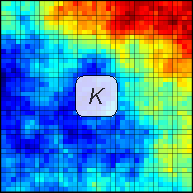
\includegraphics[width = \textwidth]{figures/perm/perm.pdf}
                }%
                \only<4->{%
                    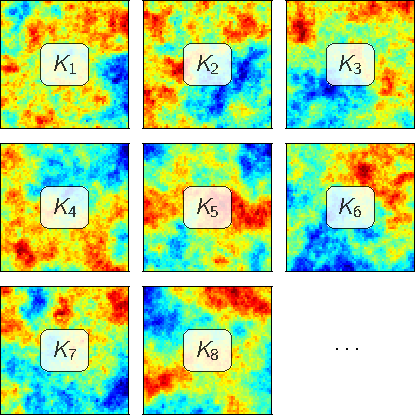
\includegraphics[width = \textwidth]{figures/perm/perm-samples.pdf}
                }%
            \end{column}
        \end{columns}
    \end{overlayarea}
\end{frame}

\begin{frame}{\name{}}
    \setlength{\cw}{0.6\textwidth}%
    \def\dx{1.5em}%
    \begin{overlayarea}{\textwidth}{\frameheight}
        \vspace{1em}%
        \textbf{Two-phase flow in porous media}
        \begin{align*}
            \partial_t(\phi S_\alpha) + \nabla \cdot \vel_\alpha = q_\alpha, \quad  \vel_\alpha = -\lambda_\alpha\perm\nabla p, \quad \alpha = w, o
        \end{align*}
        \vspace{-1.7em}
        \begin{block}{}
            \small
            \begin{center}
                $\phi$: porosity \hspace{\dx} $S_\alpha$: saturation \hspace{\dx} $\vel_\alpha$: Darcy velocity \hspace{\dx} $q_\alpha$: sources/sinks \hspace{\dx} $\lambda_\alpha$: mobility
            \end{center}
        \end{block}
        \vspace{0.3em}
        \begin{squarelist}
            \item<2-> Quantity of interest $\un$ typically derived from simulation results\only<2>{, e.g.}
            \only<2>{%
                \begin{center}
                    \small%
                    \begin{tabular}{l|l}
                        Saturation at time $t'$ & $\un = S_w(\vx, t')$ \\
                        Water production rate & $\un = q_w(t)$\\
                        Total oil production & $\un = Q_o$
                    \end{tabular}
                \end{center}
            }%
            \only<3->{\\... which are all random variables}
        \end{squarelist}
        \vspace{0.5em}
        \only<3->{
            \begin{figure}
                \centering
                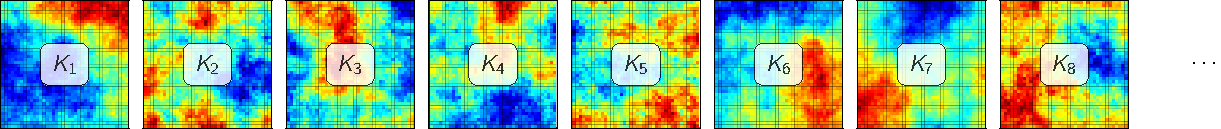
\includegraphics[width = \textwidth]{figures/perm/perm-samples-row.pdf}
            \end{figure}
        }
    \end{overlayarea}
\end{frame}

\begin{frame}{\name{}}
    \begin{overlayarea}{\textwidth}{\frameheight}
        \vspace{1em}
        \begin{squarelist}
            \item<1-> Quantity of interest $\un$ generally not scalar, but defined over domain $\Lambda$
            \begin{center}
                \small%
                \begin{tabular}{l|l|l}
                    Saturation at time $t'$ & $\un = S_w(\vx, t')$ & $\Lambda = D$ (physical domain)\\
                    Water production rate & $\un = q_w(t)$ & $\Lambda = [0,T]$ (time domain) \\
                    Total oil production & $\un = Q_o$ & $\Lambda$ not applicable
                \end{tabular}
            \end{center}
            \vspace{0.5em}
            \item<2-> Necessary substitutions with appropriate norm \redtext{$\|\cdot\|$} over $\Lambda$
            \begin{equation*}
                |\expect[\un_\ell] - \expect[\un]| \rightarrow \redtext{\|}\expect[\un_\ell] - \expect[\un]\redtext{\|}, \quad \var[\expecta_\ell] \rightarrow \expect\left[\redtext{\|}\expecta_\ell - \expect[\expecta_\ell]\redtext{\|}^2\right]
            \end{equation*}
            \item<3-> Theory for scalar variables follows directly -- particularly with \redtext{$L^2(\Lambda)$-norm}:
            \begin{equation*}
                \var\big[\expecta(\un_\nlev)\big] = \sum_{\ell = 0}^\nlev \frac{\vara_\ell}{\nsamp_\ell}, \quad \text{where } \vara_\ell = \expect\left[\redtext{\|}\expecta_\ell - \expect[\expecta_\ell]\redtext{\|}^2\right]
            \end{equation*}
        \end{squarelist}
    \end{overlayarea}
\end{frame}

\begin{frame}{\name{}}
    \renewcommand{\thealgocf}{}
    \only<1-4>{%
        \begin{algorithm}[H]
            \caption*{Multilevel Monte Carlo Method}
            \only<3>{\graytext}{%
                \textbf{Input:} Hierarchy of approximations $\ell = 0, \dots, \nlev$, tolerance $\tol$ \\
                \For(\tcp*[f]{Warmup}){$\ell = 0, \dots, \nlev$}{
                    Compute $\nsamp_w$ samples of $\un_\ell - \un_{\ell-1}$\tcp*[r]{Local MC}
                }
                Estimate $\vara_\ell$, $\cost_\ell$ and optimal $\nsamp_\ell = \nsamp_w + \nsamp_\ell'$ given desired tolerance $\tol$\\
            }%
            \only<2>{\graytext}{%
                \While(\tcp*[f]{Multilevel MC}){any extra samples needed, ($\nsamp_\ell' > 0$)}{
                    \For{$\ell = 0, \dots, \nlev$}{
                        Compute $\nsamp_\ell'$ more samples of $\un_\ell - \un_{\ell-1}$\tcp*[r]{Local MC}
                    }
                    Update estimates $\vara_\ell$, $\cost_\ell$ and optimal $\nsamp_\ell = \nsamp_\ell + \nsamp_\ell'$ given desired accuracy $\tol$ \\
                }
            }%
        \end{algorithm}
    }%
\end{frame}
\def\name{Two Illustrating Examples}

\begin{frame}{\name{}}
    \textbf{Problem}
    \begin{squarelist}
        \item The \texttt{hello world} of reservoir simulation:
        \begin{circlelist}
            \item Quarter five-spot problem with water injection in oil-filled reservoir
        \end{circlelist}
        \item Incompressible flow, linear relative permeabilities, equal viscosities
        \item Assume $\log \perm$ is Gaussian with given covariance function $\rightarrow$ 1000 realizations
    \end{squarelist}
    \visible<2->{
        \vspace{0.5em}
        \textbf{Strategy}
        \begin{numlist}
            \item Run MC simulation with 100 samples, compute RMSE $\err^{\mc}$
            \item For layer $0 \dots, L$, run 10 warmup samples to estimate $\cost_\ell$ and $\vara_\ell$
            \item Compute $\nsamp_\ell$ for desired tolerance $\tol \approx \err^{\mc}$, run and compare with MC
        \end{numlist}
    }
\end{frame}

\def\name{Example 1: Smooth Permeability}

\begin{frame}{\name{}}
    \begin{figure}
        \centering
        \only<1>{%
            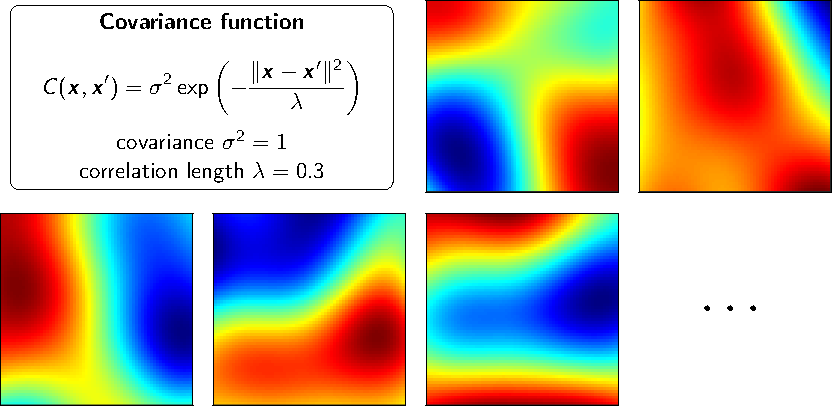
\includegraphics[width = \textwidth]{figures/example-1/perm/ex1-perm.pdf}
        }%
        \only<2>{%
            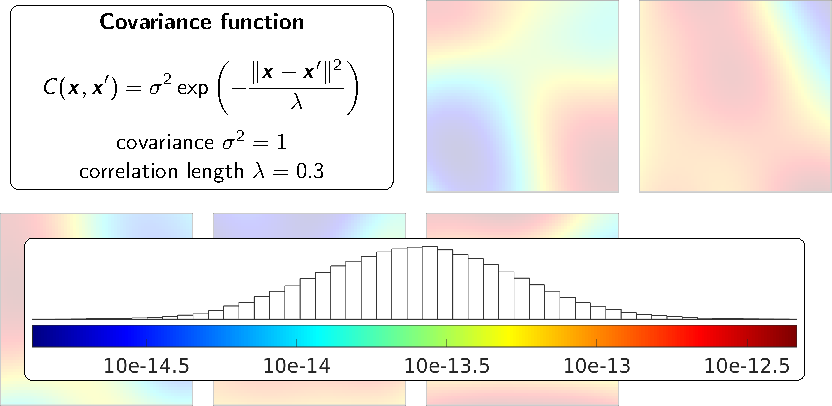
\includegraphics[width = \textwidth]{figures/example-1/perm/ex1-perm-cb.pdf}
        }%
        \only<3>{%
            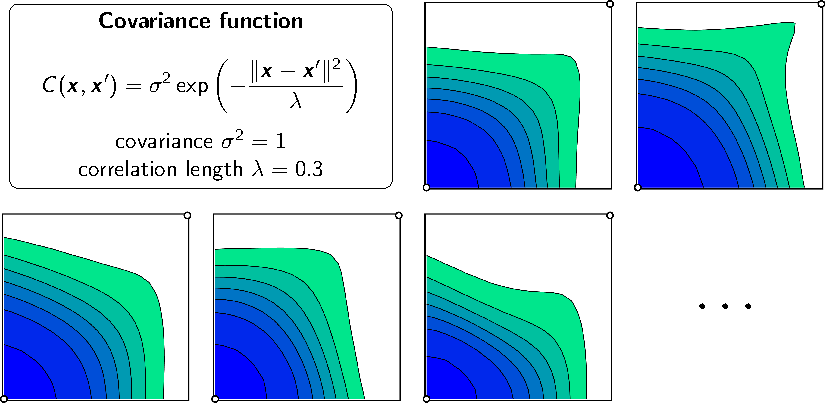
\includegraphics[width = \textwidth]{figures/example-1/sat/ex1-sat.pdf}
        }%
        \only<4>{%
            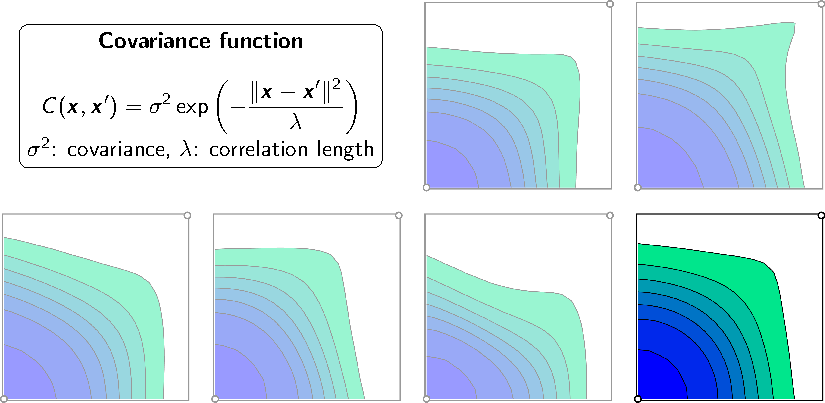
\includegraphics[width = \textwidth]{figures/example-1/sat/ex1-meansat.pdf}
        }%
    \end{figure}
\end{frame}

\begin{frame}{\name{}}
    \begin{figure}
        \centering
        \textbf{Water production rate (m$^3$/day)}
        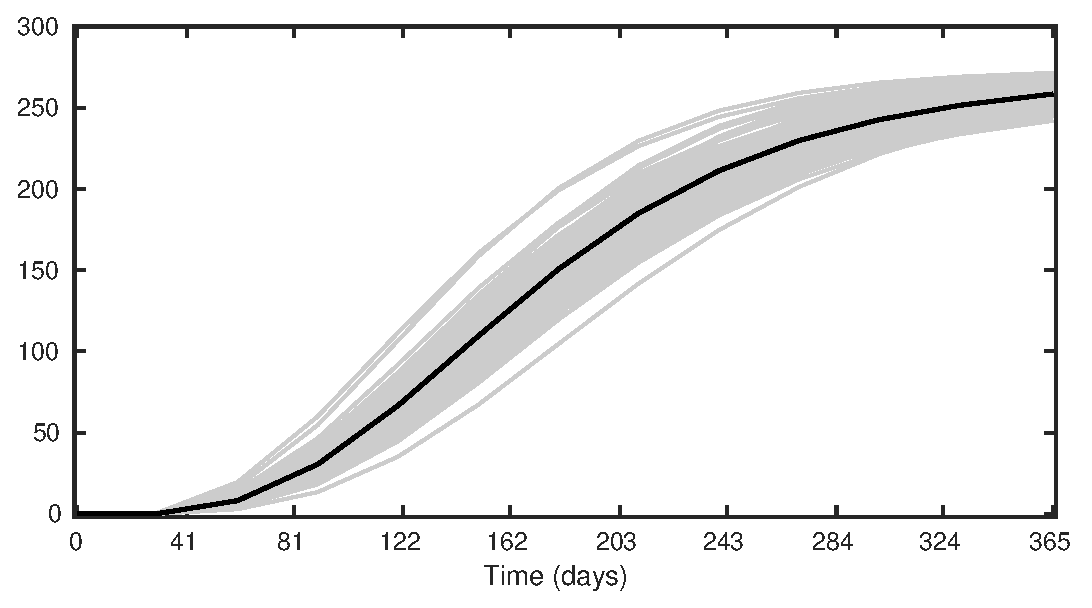
\includegraphics[width = 0.7\textwidth]{figures/example-1/water-rate.eps}
    \end{figure}
    \begin{squarelist}
        \item Monte Carlo simulation with 100 samples: $\err^\mc(q_w) = 1.0\times10^{-2}$
    \end{squarelist}
\end{frame}

\begin{frame}{\name{}}
    \begin{figure}
        \centering
        \only<1>{%
            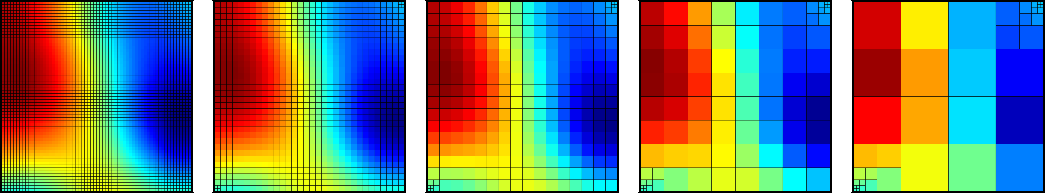
\includegraphics[width = \textwidth]{figures/example-1/permup/ex1-permup.pdf}
        }%
        \only<2>{%
            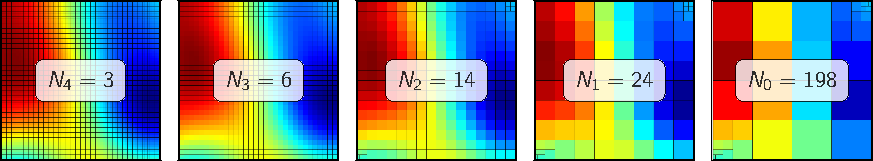
\includegraphics[width = \textwidth]{figures/example-1/permup/ex1-permup-nl.pdf}
        }%
    \end{figure}
    \begin{squarelist}
        \item<1-> Five levels with $\sim$ $4^2$, $8^2$, $16^2$, $32^2$, $64^2$ cells + refinement around wells
        \item<2-> Warmup: Run 10 samples on each level to estimate $\vara_\ell$ and $\cost_\ell$ \\
        $\rightarrow$ used to find optimal $\nsamp_\ell$ for tolerance $\tol \approx \err^{\mc}$
        \begin{equation*}
            \min\, \sum_{\ell = 0}^\nlev \nsamp_\ell \cost_\ell \quad \text{s.t.} \quad \sum_{\ell = 0}^\nlev\frac{\vara_\ell}{\nsamp_\ell} = \tol^2 \quad \rightarrow \quad \nsamp_\ell = \tol^{-2}\left(\sum_{k = 0}^\nlev \sqrt{\vara_k \cost_k}\right)\sqrt{\frac{\vara_\ell}{\cost_\ell}}
        \end{equation*}
    \end{squarelist}
\end{frame}

\begin{frame}{\name{}}
    \begin{figure}
        \centering
        \textbf{Water production rate (m$^3$/day)}
        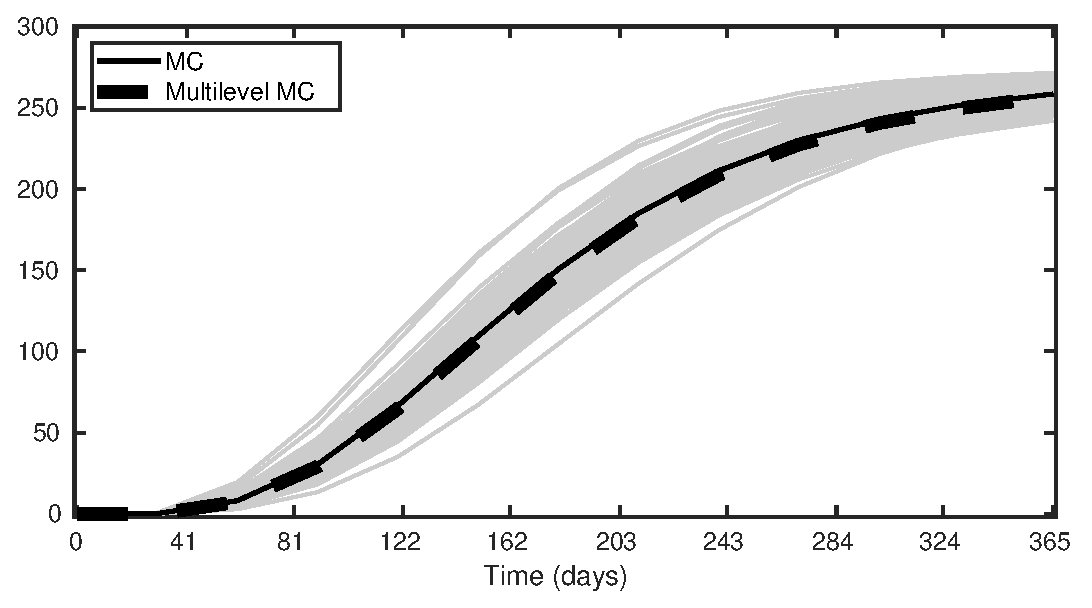
\includegraphics[width = 0.7\textwidth]{figures/example-1/water-rate-ml.eps}
    \end{figure}
    \begin{squarelist}
        \item Multilevel Monte Carlo simulation: $\err^\ml(q_w) = 1.5\times10^{-2}$
    \end{squarelist}
\end{frame}

\begin{frame}{\name{}}
    \begin{figure}
        \centering
        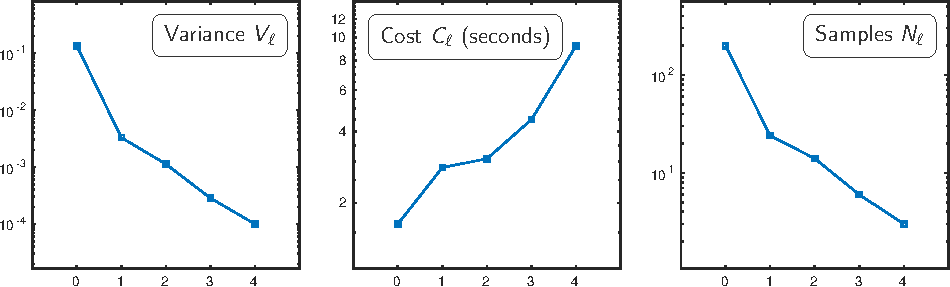
\includegraphics[width = \textwidth]{figures/example-1/statistics/ex1-statistics.pdf}
    \end{figure}
    \begin{squarelist}
        \item<2-> Total cost of Multilevel Monte Carlo: $\sum_\ell \nsamp_\ell \cost_\ell \approx 488$ s
        \item<3-> Total cost of Monte Carlo (assuming $\cost_4 = $ cost of $\un_4 -\un_3$ $\approx$ cost of $\un_4$) $\approx 923$ s\\
        $\rightarrow$ Similar accuracy with about half the cost
    \end{squarelist}
\end{frame}

% nsamples =

%      3
%      6
%     14
%     24
%   198


% c =

%     9.2327
%     4.5050
%     3.0733
%     2.8226
%     1.6266


%% run 2

% nsamples =

%      3
%      7
%     15
%     24
%   132

% c =

%     9.2925
%     4.6800
%     2.9892
%     2.6971
%     1.4028
\def\name{Example 2: Smoothly varying permeability field}

\begin{frame}{\name{}}
    \begin{figure}
        \centering
        \only<1>{%
            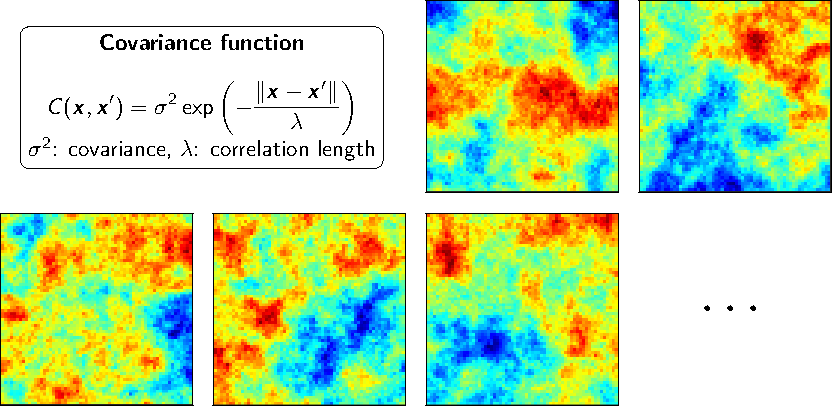
\includegraphics[width = \textwidth]{figures/example-2/perm/ex2-perm.pdf}
        }%
        \only<2>{%
            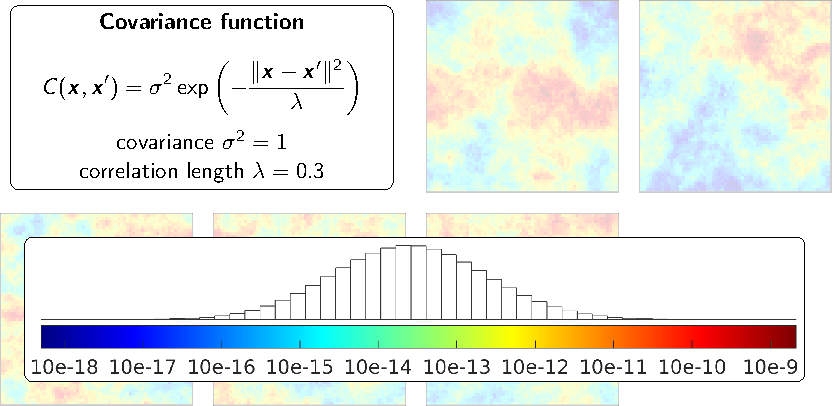
\includegraphics[width = \textwidth]{figures/example-2/perm/ex2-perm-cb.pdf}
        }%
        \only<3>{%
            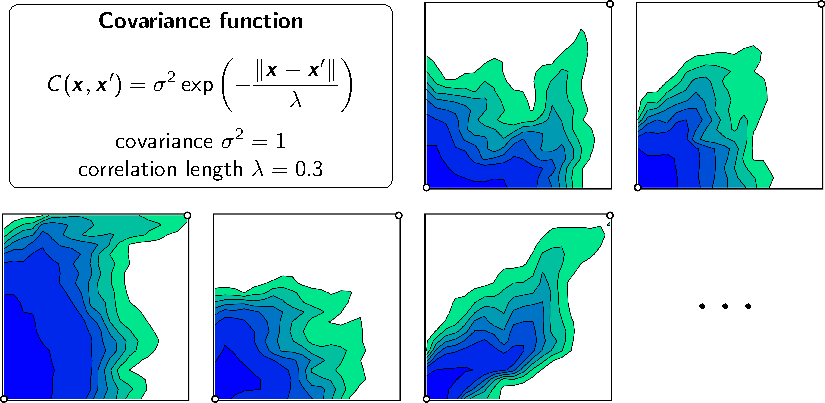
\includegraphics[width = \textwidth]{figures/example-2/sat/ex2-sat.pdf}
        }%
        \only<4>{%
            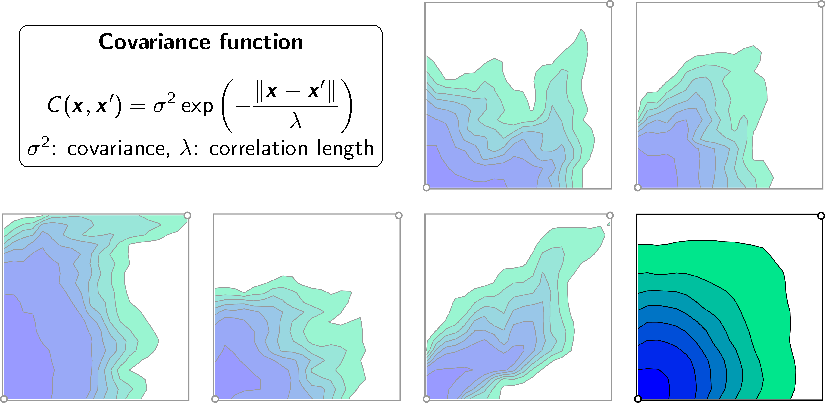
\includegraphics[width = \textwidth]{figures/example-2/sat/ex2-meansat.pdf}
        }%
    \end{figure}
\end{frame}

\begin{frame}{\name{}}
    \begin{figure}
        \centering
        \textbf{Water production rate (m$^3$/day)}
        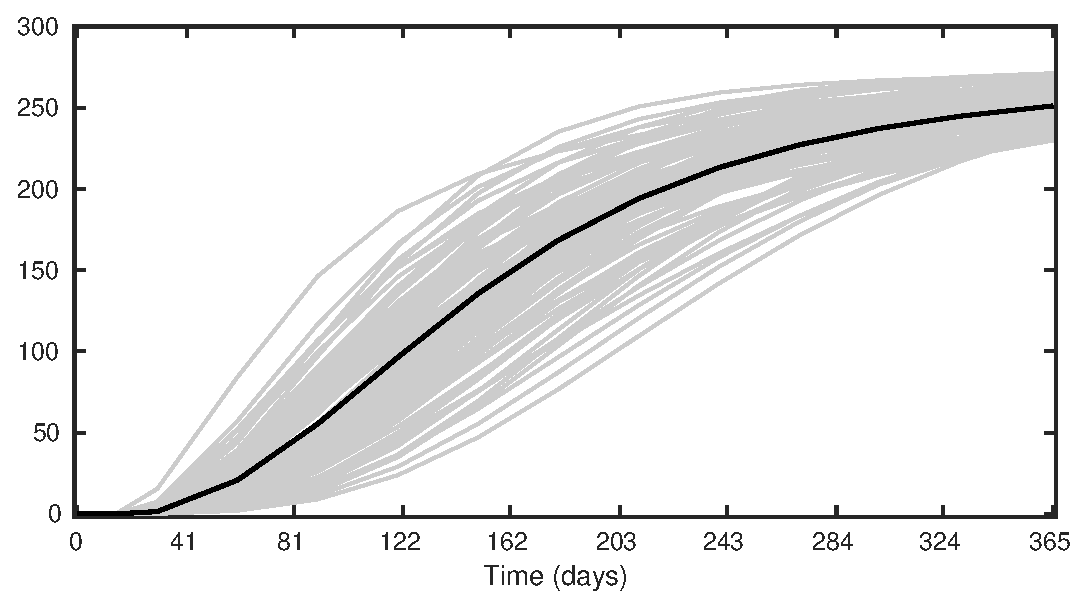
\includegraphics[width = 0.7\textwidth]{figures/example-2/water-rate.eps}
    \end{figure}
    \begin{squarelist}
        \item Monte Carlo simulation with 100 samples: Total variance $\err^\mc(q_w) = 1.1\times10^{-4}$
    \end{squarelist}
\end{frame}

\begin{frame}{\name{}}
    \begin{figure}
        \centering
        \only<1>{%
            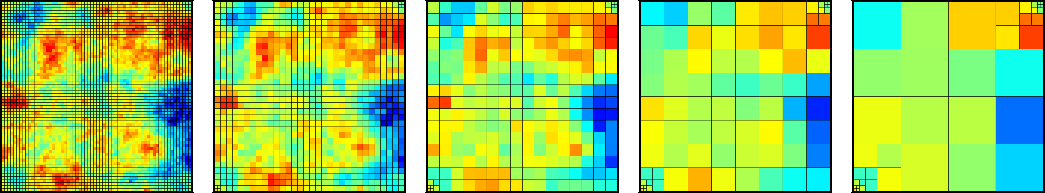
\includegraphics[width = \textwidth]{figures/example-2/permup/ex2-permup.pdf}
        }%
        \only<2>{%
            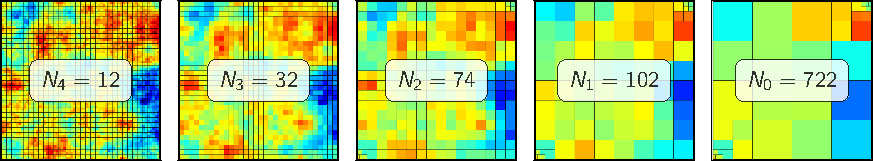
\includegraphics[width = \textwidth]{figures/example-2/permup/ex2-permup-nl.pdf}
        }%
    \end{figure}
    \begin{squarelist}
        \item<1-> Five levels with $\sim$ $4^2$, $8^2$, $16^2$, $32^2$, $64^2$ cells + refinement around wells
        \item<2-> Warmup: Run 10 samples on each level to estimate $\vara_\ell$ and $\cost_\ell$ \\
        $\rightarrow$ used to find optimal number of samples
        \begin{equation*}
            \min\, \sum_{\ell = 0}^\nlev\frac{\vara_\ell}{\nsamp_\ell} \quad \text{s.t.} \quad \cost = \sum_{\ell = 0}^\nlev \nsamp_\ell \cost_\ell \qquad \rightarrow \cost = \tol^{-2}\left(\sum_{\ell = 0}^\nlev \sqrt{\vara_\ell \cost_\ell}\right)^2, \quad \nsamp_\ell = \lambda\sqrt{\frac{\vara_\ell}{\cost_\ell}}
\end{equation*}
    \end{squarelist}
\end{frame}

\begin{frame}{\name{}}
    \begin{figure}
        \centering
        \textbf{Water production rate (m$^3$/day)}
        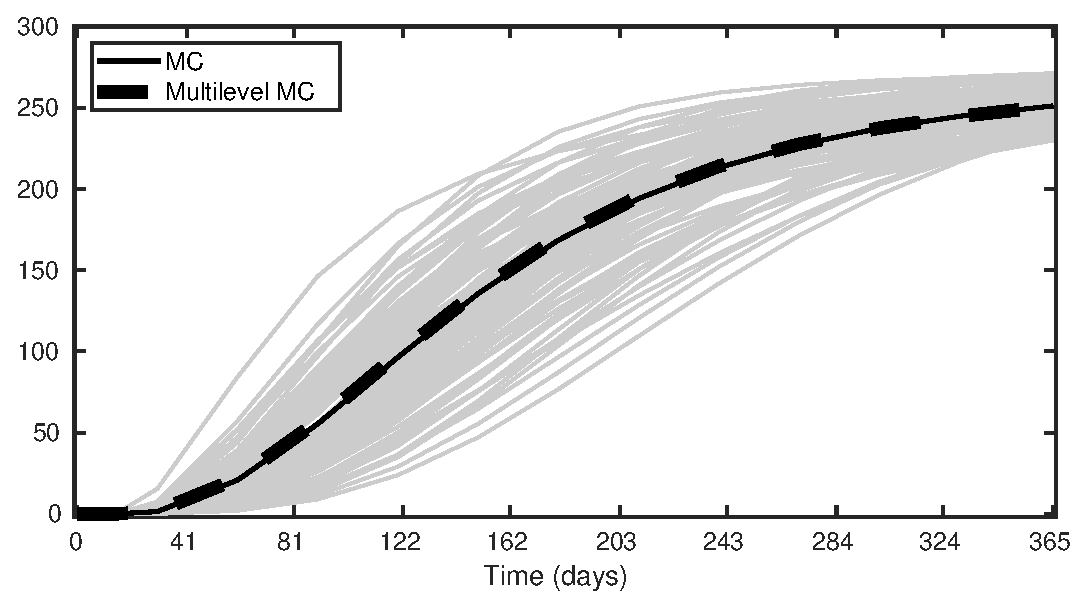
\includegraphics[width = 0.7\textwidth]{figures/example-2/water-rate-ml.eps}
    \end{figure}
    \begin{squarelist}
        \item Multilevel Monte Carlo simulation: Total variance $\err^\ml(q_w) = 1.4\times10^{-4}$
    \end{squarelist}
\end{frame}

\begin{frame}{\name{}}
    \begin{figure}
        \centering
        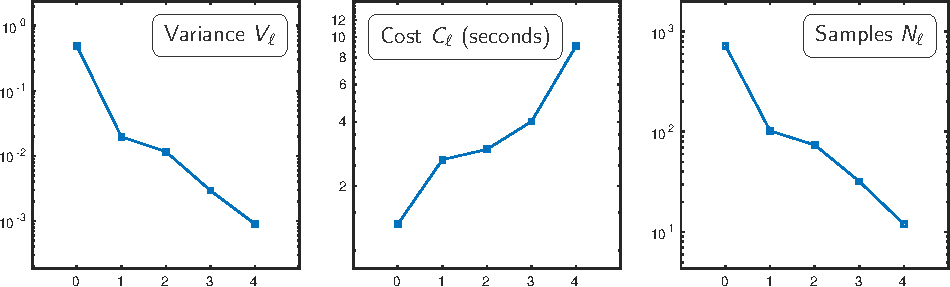
\includegraphics[width = \textwidth]{figures/example-2/statistics/ex2-statistics.pdf}
    \end{figure}
    \begin{squarelist}
        \item<1-> Total cost of Multilevel Monte Carlo: $\sum_\ell \nsamp_\ell \cost_\ell \approx \only<2>{\redtext}{1686}$ s
        \item<2-> Total cost of Monte Carlo (assuming $\cost_\nlev = $ cost of $\un_4 -\un_3$ $\approx$ cost of $\un_4$) $\approx 909$ s
    \end{squarelist}
\end{frame}

\section{Concluding Remarks}
\def\name{Concluding Remarks}

\begin{frame}{\name{}}

    \textbf{A few pitfalls and shortcomings}\vskip2mm
    \begin{squarelist}
        \item<2-> Convergence theory with conditions in terms of unknown quantities
        \begin{circlelist}
            \item Number of samples needed to approximate $\vara_\ell$, $\cost_\ell$ is problem-dependent
        \end{circlelist}
        \item<3-> Use upscaling with care
        \begin{circlelist}
            \item Coarsest level $\ell = 0$ should have cell diameter $h \sim$ correlation length $\lambda$
        \end{circlelist}
        \item<4-> Very challenging to upscale complex models in a meaningful way
        \begin{circlelist}
            \item Channelized reservoirs, different rock types, multiphase, etc. \\
            ... and the best methods are expensive
        \end{circlelist}
        \item<5-> Not all choices of $\un$ are appropriate!
        \begin{circlelist}
            % \only<3-5>{%
            %     \item<4-5> Example: saturation at specific point and time
            %     \item<5-5> Example: binary output $\un \in \{0,1\}$ (e.g., fracture propagation)
            %     \begin{equation*}
            %         \un_\ell - \un_{\ell-1} = 
            %         \begin{cases}
            %             1 & \text{probability $p$} \\
            %             -1 & \text{probability $q$} \\
            %             0 & \text{probability $1-(p+q)$}
            %         \end{cases}
            %         \quad p,q \ll 1 \rightarrow \expect[\un_\ell - \un_{\ell-1}] \approx 0
            %     \end{equation*}
            % }%
            \item Rule of thumb: average of $\un$ should ''make sense'' for the problem at hand
        \end{circlelist}
    \end{squarelist}
    
\end{frame}

\begin{frame}{\name{}}

    \textbf{Can we do better?}\vskip2mm
    \begin{squarelist}
        \item<2-> \emph{Level} does not necessarily mean spatial resolution!
        \begin{circlelist}
            \item Solver-based: use a more accurate solver for higher levels\\
            e.g., increasing accuracy of spatial/temporal discretization with level
            \item Multiscale methods (compromise between upscaling and solver accuracy)
        \end{circlelist}
        \item<3-> MLMC does not require a geometric sequence of levels 
        \begin{circlelist}
            \item Sufficient that accuracy and cost \emph{increase} and variance \emph{decrease} with $\ell$
        \end{circlelist}
        \item<4-> Multi-index Monte Carlo -- change multiple aspects of simulation with
        level
        \begin{circlelist}
            \item Example: resolution in space \emph{and} time, $\ell \rightarrow \vect \ell = (\ell_{\vx}, \ell_t)$
        \end{circlelist}
        % \item<7-> Richardson extrapolation -- more accurate estimates of $\un_\ell - \un_{\ell-1}$
    \end{squarelist}
    
\end{frame}

\def\name{Suggested Literature}

\begin{frame}{\name{}}
	\begin{scriptsize}
    	\bibliography{refs}
	\end{scriptsize}
\end{frame}

\begin{frame}
    \vspace{1em}
    \begin{block}{}
        \small
        Developed by nuclear physicist Stanislaw Ulam during the Manhattan Project in the late 1940's\vskip5mm
        {\itshape It was at that time that I suggested an obvious name for the statistical method -- a suggestion not unrelated to the fact that Stan had an uncle who would borrow money from relatives because he "just had to go to Monte Carlo"}\vskip5mm
        \hspace*\fill{\small--- Nicholas Metropolis, {\itshape The Beginning of the Monte Carlo Method} (1987)}
    \end{block}
\end{frame}

\end{document}
